\section{Related Work}
\label{state:related}

This section presents prior work and puts emphasis on the parts pertinent to
this work.
One assumption for this work is already in place:
the target architecture is a single ISA, partly symmetric homogeneous
multicore.
Partly symmetric means the target architecture supports \gls{smt},
but besides this, it is a \gls{smp} architecture.
Hence, research proposing hardware changes, e.g. \cite{cruz_dynamic_2014},
are out of scope.
Also research focusing on heterogeneous or multi-ISA architectures, e.g.
\cite{sarma_smartbalance_2015}, are not part of the review.

%One restriction applies to this review: mechanism proposing hardware changes
%are not in the focus of this work.
%This restriction excludes interesting ideas to gather behavioural information,
%e.g. observation of cache coherency traffic proposed in
%\cite{cruz_dynamic_2014}.


In literature, different approaches to load balancing on a multicore have been
explored.
\citeauthor{snavely_symbiotic_2000} introduced the term \emph{symbiotic
scheduling} in \cite{snavely_symbiotic_2000}, describing a scheduling technique
for \gls{smt}-systems.
They propose scheduling these two jobs on a shared core, which provide the best
utilization of said core.
The combination of two jobs on two corresponding \gls{smt}-cores call they a
co-schedule.
The performance of a co-schedule is defined as the turnaround or response time:
the time between the arrival of a job in the system and its completion.

In their experiments they run independent jobs on a simulator modeling a Compaq
Alpha 21264 out-of-order processor with hardware additions for multi-threading.
This simulator model includes performance counters to ``capture dynamic execution
information''(\autocite[236]{snavely_symbiotic_2000}).
To determine a good schedule they compute the weighted speedup \textit{WS} for
a fixed time interval.
For each job the change in instructions per cycle (IPC) compared to
single-threaded execution is calculated.
The sum of these values for all jobs is the weighted speedup of this
schedule.
$$ WS(t) = \sum_{i=1}^n (\text{realized IPC job}_i / \text{single-threaded IPC
job}_i)$$
Their developed scheduler consists of two phases: sampling and symbiosis.
During the sampling phase different job combinations are measured.
When enough samples are gathered, the scheduler moves to the symbiosis phase
and uses schedules, which promise the highest weighted speedup.
The scheduler will move back and forth between these phases, as the job-mix
changes.

The measurements of the performance counters are used to create several
predictors for the behaviour of jobs in the future and, hence, the best schedule.
The best predictor in their study made a majority vote of all other predictors
to determine the best schedule.
\citeauthor{snavely_symbiotic_2000} conclude, that good job symbiosis depends
not only on high IPC, but on several behavioural factors.
\\


In \citeyear{snavely_symbiotic_2002} \citeauthor{snavely_symbiotic_2002}
discussed the topic of priorities in symbiotic schedules.
In their earlier work (\cite{snavely_symbiotic_2000}) they assumed same
priority jobs.
Now, they present two meanings for priority: ``(A) guarantee a fraction of
machine proportional to priority'' or ``(B) guarantee a fraction of
single-threaded performance proportional to priority''
(\autocite[70]{snavely_symbiotic_2002}).
The authors base their priority mechanisms on two values: SOLOFRAC and CS.
SOLOFRAC is the from the priority derived fraction of the CPU time,
a job needs to be scheduled alone  and CS is the fraction of the CPU time,
where no job is solo scheduled.

The \textit{Naive} priority mechanism schedules a job alone for its SOLOFRAC
share and co-schedules for CS cycles. Behind this stand two assumptions: first,
during co-scheduling each job is an equal share of the cycles assigned.
And second, the number of jobs does not exceed the number of \gls{smt}-cores.

The proposed \textit{Symb} mechanism on the other hand, can handle more jobs
than available \gls{smt}-cores and observes job behaviour. By running jobs
solo, it determines the job's ``'natural' IPC''
(\autocite[71]{snavely_symbiotic_2002})
and can evaluate the job's performance during a phase of co-scheduling.
Based on this measurement, the SOLOFRAC is reduced such that the job get its
rightful share of cycles. The increase in co-scheduling time leads to increased
utilization of the system.

Other presented approaches in \cite{snavely_symbiotic_2002} require hardware
changes and are therefore out of scope.
\\

While \citeauthor{snavely_symbiotic_2000} claim in
\cite{snavely_symbiotic_2000} a reduction in average turnaround time by up to
17\%, \citeauthor{eyerman_revisiting_2015} state a mere 3\% to 6\% increase in
average throughput with an optimal symbiotic scheduler compared to a
first-come-first-serve scheduler.
The notable difference explain the authors in \cite{eyerman_revisiting_2015} as
different experimental views. \citeauthor{snavely_symbiotic_2000} study a fully
loaded system with twice as much ready jobs as SMT-cores and observe the
turnaround time.
The turnaround time of a job is mainly influenced by the time it waits in the
ready queue, when all cores are loaded.
If the maximum throughput increases slightly, the waiting time is reduced,
hence, a significant reduction in turnaround time is observed.
Also a job reordering in a shortest remaining time first manner, can also
reduce the average turnaround time.
For these reasons \citeauthor{eyerman_revisiting_2015} make the case,
that turnaround time alone can be a misleading measure.

Furthermore, maximum throughput cannot be used, because systems are not
designed to run at peak load all the time, as this leads to long queues and
turnaround times.
Average throughput equals average load, if the system is not fully loaded,
therefore, it is a useless comparator.
Instead, they advocate to evaluate processor utilization (understood as average
number of executing cores) and empty periods.
If throughput is improved, the processor utilization decreases and empty
periods are enlarged, as the time to execute the current load is reduced.
Hence, using these two measures scheduler caused improvements can be compared.

\citeauthor{eyerman_revisiting_2015} conclude that one should not expect large
improvements through symbiotic scheduling, but particular workloads my benefit.
Furthermore, previous studies on partially symmetric mutlicores showed
substantial throughput gains by symbiotically co-scheduling applications on
SMT-packages.
\\


\citeauthor{banikazemi_pam_2008} present a study concerning thread-to-core
mappings on partially symmetric multicores.
In \cite{banikazemi_pam_2008} they present \emph{PAM}: a performance/power-aware
meta-scheduler, working on top of the default Linux scheduler.
While the default scheduler runs, PAM gathers information via performance
counters on cache occupancy, cycles per instruction, and the miss ratio of L1
and L2 caches for each thread.
If PAM can predict a better thread-to-core mapping, based on this information,
it overrules the default scheduler and enforces the better mapping.
With a \textit{Goodness(t)} metric PAM rates the current mapping for the last
time interval.
Depending on the goodness value of the PAM mapping being better than the one of
the default scheduler, PAM continues to enforce its mapping or falls back to
default.
Goodness can be describing performance, power or energy consumption.

The experiments ran on a dual socket, quad-core machine, where two cores
share an L2 cache, making this a \gls{cmp} approach.
The processor does not support \gls{smt}.
Hence, the improvement gains stem not from symbiosis, but rather from
congestion awareness.
\\

Reducing cache congestion was the main point in \cite{knauerhase_using_2008}.
Like \citeauthor{banikazemi_pam_2008}, they worked on a \gls{cmp}-machine with
two separated cache groups sharing an L2 cache.
Similarly, they tried to spread memory intensive tasks as much as possible,
to reduce interference in the shared cache.
They introduce the metric called cache weight, which terms the \gls{llc}-cache
misses per cycle for the last time interval.
Their research showed, that longer histories worsen the prediction, as thread
behaviour changes over time.
To achieve the best possible spread of all threads across cache groups,
\citeauthor{knauerhase_using_2008} balance the threads in the \gls{llc}-group
based on the aggregate cache weight.
New threads are assigned to the cache group with the lowest weight and only
cache light tasks are migrated across group boundaries.
However, to care for workload changes, an overweight thread is periodically
migrated to the lightest \gls{llc}-group.
Cache light threads suffer next to cache intensive threads, as they most likely
start with a cold cache, each time they are scheduled.
To compensate this, \citeauthor{knauerhase_using_2008} propse to transfer CPU
time from the cache heavy to the suffering threads.
This fairness compensation reduced the performance degradation of the most
suffering thread to less than 1\%.
\\


But \gls{cmp} and \gls{smp} systems share more resources than just the cache.
In \cite{fedorova_managing_2010}, \cite{zhuravlev_addressing_2010}, and
\cite{zhuravlev_survey_2012} \citeauthor{fedorova_managing_2010} and
\citeauthor{zhuravlev_addressing_2010} further investigate congestion on shared
resources.
Although their assumption in \cite{fedorova_managing_2010} was, that memory
reuse patterns are the indicator of
choice to predict cache interference between threads, their research lead to
the conclusion that \gls{llc}-misses are superior.
Memory reuse patterns model the access frequency of a memory area and the miss
frequency for a particular application.
This analysis has to be done off-line and assumes, that applications with high
reuse and low miss rates, do not affect other applications negatively, but
applications with low reuse and high miss rates are likely to trash the cache
of others.
To do this on-line the authors derived a metric called \emph{Pain}, which
consists of two parts: sensitivity and intensity.
The former describes how much an application suffers from sharing caches with
others, the latter how much an application will hurt others.
The pain application A feels when scheduled with B is the product of A's
suffering and B's intensity.
Vice versa for B.
The sum of both describes the expected performance degradation for these two
applications, when being scheduled together on the same \gls{llc}.
To approximate sensitivity and intensity on-line they assumed cache miss and
access rates would be a good measure, but it turned out only the cache miss
rate is relevant.
The memory reuse patterns only focus on the cache as shared resource.
The cache miss rate on the other hand also predicts the load on prefetching
hardware, memory controller and front side bus.
Load on these shared resources showed to be the main reason for performance
degradation in most of their benchmarks (\cite{zhuravlev_addressing_2010}).
\\

However, they all assumed independent, non-interacting threads.
\citeauthor{hofmeyr_load_2010} present in \cite{hofmeyr_load_2010} a load
balancing technique explicitly assuming interacting, parallel applications.
They propose a technique called \emph{speed balancing} with a notion for fast
and slow cores.
They assume an oversubscribed environment, where the number of runable threads
is greater than the number of cores.
Fast and slow cores are determined by run queue length.
Thread progress is slower on longer queues, hence, slow cores are cores with a
longer run queue.
The term speed is defined as the relation of execution time per elapsed wall
clock time.
The speed of each thread determins, if it is running on a fast or a slow core.
The algorithm presented by \citeauthor{hofmeyr_load_2010} runs one thread per
core producing a speed measure for each thread and the core respectivly.
To compare core speeds, a global average core speed is computed.
To provide equal progress oportunities, each thread needs to run on a fast
core at least once.
Hence, the balancing thread on a fast core searches for a suitable thread to
migrate from a slow core and pull it to its local core.
Thereby, the balancing thread tries to migrate the least migrated thread to
avoid constant migration of the same thread.

The parallel application model the authors assume consists of one application
spawning several worker threads, where a computation interval is followed by a
communication barrier.
Their implementation takes this application as input, executes it and provide
equal progress to each thread.
They do neither model communication between unrelated tasks in a client-server
notion, nor at arbitrary points in time.
Hence, reducing the time the slowest thread needs to reach the synchronization
point improves overall application performance.

\todo{linux cfs scheduler}


% -----------------------------------------------------------------------------

\section{Fiasco.OC \& L4Re}
\label{state:env}
\todo{Fiasco.OC \& L4Re}

\textbf{Fiasco.OC}
\begin{itemize}
  \item Kernel scheduler does no balancing, assigns thread to the first
    core specified in the affinity descriptor
  \item affinity descriptor: core(s) a thread should run on
  \item Syscall via run\_thread() to pass affinity descr to kernel scheduler
  \item interface to query execution time for each thread \todo{difference
      between execution time and cycles? Cycles project changes in core speed
      due to turbo boost or other mechanism}
  \item	todo: Performance counters
  \item capability system
\end{itemize}

\textbf{L4Re}
\begin{itemize}
  \item provides scheduler proxy interface, including affinity descriptor,
    scheduling parameters
\end{itemize}


% -----------------------------------------------------------------------------

\section{\gls{intel} Haswell Architecture}
\label{state:haswell}

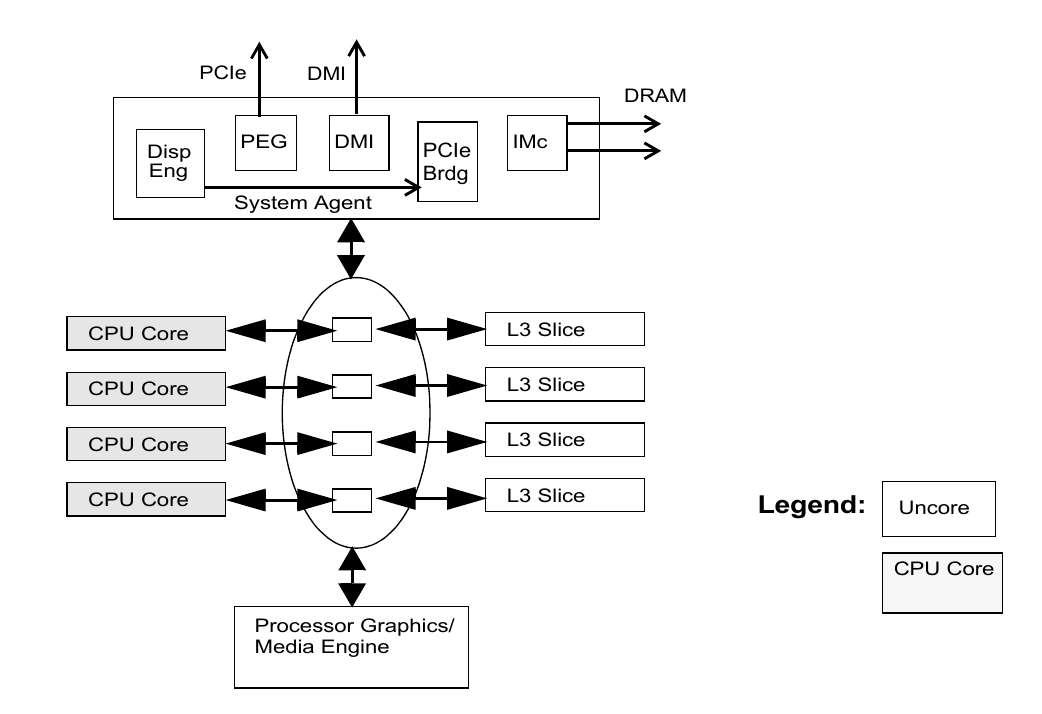
\includegraphics[width=0.8\textwidth]{images/haswell_architecture_by_intel_large}

\includegraphics[width=0.8\textwidth]{images/haswell_core_layout}


\begin{itemize}
  \item diagram of architecture: four cores with L1I/D \& L2 cache; two smt/ht
    cores per physical core; L3 cache shared and sliced, ring buffer for
    access; mem controler in uncore package;
  \item 4 prefetcher per cache; 2 for L1D, 2 for L2 cache
  \item L1D \& L2 cache data is present in L3 cache to be able to redirect
    requests from other cores to the correct cache. --> Issue with security; no
    cache side attack surface reduction
  \item IF security: dual socket system with one core dedicated to security
    tasks for an interval
  \item L3 cache slices corespond to number of cores
  \item logic portion and data array portion; access, coherency, memory
    ordering, LLC misses, writeback to memory; cache lines
  \item hash function uniformly distributes addresses
  \item access times to L3 cache varies depending on travel distance on the
    bi-directional ring buffer
  \item system agent receives memory requests not serviced by cache and
    redirects to IMC
\end{itemize}

\paragraph{Issues with security core idea:}
The idea to reduce attack surface for e.g. openssh cache attacks was to provide
a dedicated core for security critical applications.
This idea spawned from the assumption that L1D \& L2 cache was solely present
on a core, but the L3 cache content is a superset of all cores L1D \& L2 cache.
Hence, cache side channel attacks are still possible, although more
complicated, as the attacker not present on the core, must determine, which
cache lines correspond to the L1D \& L2 cache of the ``security core''.
Attacks presented in \cite{yarom_recovering_2014} and
\cite{bernstein_cache-timing_2005} rely on the fact, that only one application
is using cache lines on the core.
On a multicore, only observing the \gls{llc}, other running applications will
disturb the observations, effectivly reducing the side channel throughput.
\todo{This should be part of the architecture chapter, as the security core
idea wasn't presented yet.}

% -----------------------------------------------------------------------------

\section{Contribution}
\label{state:contr}


\begin{itemize}
  \item Current processor architectures don't use CMP processors any more, therefore
    the cache layout is different. My work evaluates the research results on the
    new HW layout. But AMD Opteron Barcelona had a similar cache layout.
  \item User level scheduling on a $µ$-kernel. But user level scheduling was
    done before.
  \item More scheduling parameters \textit{or} less assumptions about threads.
  \item No off-line measurements, only on-line information gathering.
  \item Thread interaction possible (communication partner, security flag)
  \item Designated cores for security critical applications.
\end{itemize}


% -----------------------------------------------------------------------------

\begin{comment}
\begin{itemize}
  \item Assumptions: single ISA, no heterogeneous cores, SMP, one specific CPU
    architecture \checkmark
  \item Goals: load balancer providing isolation, stable execution times for the
    same workload, reduced congestion on shared resources, two balancing
    strategies: performance and low energy usage;
  \item introduce different approaches: speed balancing, symbiotic scheduling,
    congestion aware scheduling

    \begin{itemize}
      \item concisely introduce the work
      \item highlight the key aspects, goals, achievements
      \item relevant achievements I will use
      \item drawbacks of the work
    \end{itemize}
  \item symbiotic scheduling:
    \begin{itemize}
      \item term coined by \citeauthor{snavely_symbiotic_2000} in
	\citeyear{snavely_symbiotic_2000} \checkmark
      \item technique for SMT to improve performance of threads scheduled on
	two hardware sharing SMT cores \checkmark
      \item runs threads on two corresponding SMT cores and measures their
	performance in a simulator;
      \item explain performance, turnaround/response time. How measured?
	\checkmark
      \item sampling phase needs time, but can be done, while a default
	scheduler runs \checkmark
      \item restriction on changes in workload to ease sampling phase
      \item summarize all restrictions/assumptions
      \item select thread pairs/co-schedules for smt-core-pairs with most throughput for
	all threads
      \item try to combine workloads that use different cpu hardware
	units, e.g. fp workload and integer workload; heavy cache usage, little
	cache usage
      \item Measurements in their \citeyear{snavely_symbiotic_2000} paper use
	perf counters not present in real HW, e.g. conflicts inside FP units,
	FPqueue full.

      \item  \citeauthor{snavely_symbiotic_2002}: simulator, no real hardware,
	but priority sensitive (2002) \checkmark
      \item priority is perceived as ``guarantee a fraction of machine
	proportional to priority'' or `` guarantee a fraction of
	single-threaded performance proportional to priority'' \checkmark
      \item can it also be seen as a guarantee, that no lower priority thread is
	scheduled unless I have been selected to run? Can I guarantee that in a
	multicore setup, without knowledge of the execution times? -> No.
	\todo{is an example beneficial here?}
	I can just guarantee, that the plan based on the prediction cares for
	priorities.

      \item \citetitle{eyerman_revisiting_2015}: symbiotic scheduling does only
	provide an average throughput gain of around 3%.
      \item reason: the most test case assumptions in literature are beneficial
	for symbiotic scheduling, but not close to reality.
      \item gather all information for a optimal scheduler with total knowledge
      \item theoretical optimal schedule knows the performance of all tasks in
	all possible combinations with all other tasks.
      \item use simulator to measure tasks on a 'reference core' and
	compute throughput and IPC values for different schedules.
      \item First-come-first-served scheduler is close to the theoretically
	optimal scheduler
      \item arrival time of tasks is critical for FCFS schedule throughput and
	hence determines, how close FCFS comes to the optimal scheduler
      \item difference in experiments: turnaround time reduction in latency
	experiment(\cite{snavely_symbiotic_2000}) vs. average throughput in a
	maximum throughput experiment (\cite{eyerman_revisiting_2015}).
      \item processor utilization or empty time are better indicator of
	scheduler efficiency than only presenting turnaround time, best use all
      \item compare scheduler by comparing these three indicators
      \item overload situations := job arrival > max throughput
      \item besides FCFS scheduler all other need an off-line phase to measure
	the jobs, to be able to determine an optimal co-schedule.
    \end{itemize}

  \item congestion aware scheduling
    \begin{itemize}
      \item goal: minimizing usage of shared hardware resources
      \item shared hw resources are: shared caches, prefetching hardware, bus
	and memory controller
      \item options: cache line reuse / memory reuse pattern vs. miss rate
      \item \citeauthor{fedorova_managing_2010} started out with cache line
	reuse and came to the conclusion, that the off-line measurement of
	memory reuse pattern and conclude, that this is not the best approach
	to approximate congestion.
      \item they develop a PAIN metric, combining sensitivity and intensity
	concerning shared cache usage: sensitivity: how much do I suffer by
	shared cache; intensity: how much do I hurt others;
      \item off-line measurement possible, but what is a good on-line
	approximation? Cache-miss rate and cache-access rate? (Intuitively
	correlate with intensity and reuse frequency)
      \item evaluation shows best on-line approximation for pain metric is LLC
	miss rate: combines sensitivity and intensity
      \item miss rate expresses load on FSB, prefetching hardware and
	mem controller, which are the main cause for performance degradation,
	not the cache. (what is PAMs cache occupancy ratio worth now?)
      \item ``An application aggressively using prefetching hardware will also
	typically have a high LLC miss rate, because prefetching requests for
	data that is not in the cahce are counted as cache misses. Therefore, a
	high miss rate is also an indicator of the heavy use of prefetching
	hardware.'' (\cite{fedorova_managing_2010}).

      \item \cite{knauerhase_using_2008} use LLC-misses as predictor
	for cache interference and attempt to keep the sum of cache
	weights/LLC-misses of all running processes close to a medium value
      \item they also use task behaviour of the last time quantum as predictor
	for the behaviour in the next; temporal locality predictor.
      \item migration across cache borders: avoid migrating overweight/ high
	cache impact tasks, try to balance cache groups by migrating small
	tasks (assuming CMP architecture). How high is the impact, if LLC is
	shared anyway?
      \item periodically, migrate overweight task to find a possibly better
	load distribution
      \item fairness: give cache light tasks, that suffer a lot due to being
	scheduled next to cache intensive tasks, bonus execution time.
      \item assumed independent jobs

      \item \citetitle{banikazemi_pam_2008}: use real CMP system: 8 core two
	socket IBM Blade
      \item use symbiotic approach on CMP systems, less shared HW, no SMT
      \item relies on Linux scheduler as default
      \item only when better performing thread-to-core mapping is predicted, the
	default scheduler is overruled for a defined count of scheduling-cycles
      \item uses hardware performance counter evaluate and support decisions
      \item goodness metric to rate the thread-core-mapping if not better than
	last goodness rating of default scheduler, fall back to default
	scheduler
      \item mathematical model for the algorithm
      \item measured parameters are cache occupancy ratio, cycles per
	instruction, L1	and L2 miss ratio
      \item compute performance estimation for selected plan
    \end{itemize}

  \item security relevance of shared resources
    \begin{itemize}
  \item cache side channel attacks undermining security of OpenSSL; how thread
    placement minimizes side channel surface;
    \end{itemize}

  \item what is relevant and will be used, where improves this work the
    previous (contribution)
  \end{itemize}

\paragraph{ \cite{sarma_smartbalance_2015} }
\citeauthor{sarma_smartbalance_2015} write about their approach to balance work
in a heterogeneous system.
They assume a system with a single ISA and several CPUs with different performance
characteristics and different hardware features.
\todo{check different hw features}
They introduce categories for each performance level and measure the
performance differences between each level.
This results in a matrix displaying the performance gain or degradation, when
a work package (e.g. thread) is migrated.
Their load balancing algorithm has three phases: sense, predict, balance.
During the sense phase the algorithm observes the CPU utilization for an intervall.
An intervall consists of configurable many clock ticks.
The sense-result is then used by the prediction phase to compute a load
expectation for the different performance levels.
Based on this forecast a balancing decision is made and enforced in the third
phase.
Their model can also select the best CPU size for a optimal performance per
joule ratio.

\textbf{relevant} load balancing algorithm: sense, prediciton, balance,
intervall;

\textbf{not} heterogeneous processors, gem5, big.LITTLE, performance
matrix;

\paragraph{ \cite{hofmeyr_load_2010} }
evenly distributed run\_queues are assumed, slow cores are cores with longer
queues than others.

\textbf{relevant} notion of speed of a processor: $speed = t_{exec}/t_{real}$;
sched\_setaffinity to migrate threads; PIDs of all the threads of a task;
core speed computation and comparison algorithm;
distributed balancing thread with global synchronization;
assumptions \& drawbacks of kernel level load balancing;
in oversubscibed environments balance trumps locality;
\textbf{assume interacting tasks}


\textbf{be aware} turbo boost -> different core speeds on same CPU;
sched\_yield and sleep difference: run queue;

\textbf{not} NUMA, MPI, OpenMP;

\textbf{shortcommings} Tigerton: no \gls{ht}, no turbo-boost, no l3 cache,
and a dual-die CMP architecture.


\paragraph{ \cite{zhuravlev_survey_2012} }
\citeauthor{zhuravlev_survey_2012} provide a survey over scheduling techniques,
aiming at better usage of shared resources in multicore processors.
They focus on \gls{cmp}s, which share caches between at
least two cores, but not between all cores.
Techniques like hyper-threading are also taken into account.
\todo{redo this section, cmp, smp already in terminology}
Simultaneous multiprocessors (SMPs) are not in the focus of their survey.
\gls{intel} newer architectures, e.g. Haswell, is a \gls{smp} architecture, where each
physical core has dedicated L1 \& L2 caches, but the L3 cache is shared between
all cores.
Their algorithmic focus lies on contention-aware schedulers, which consists of
four building blocks: objective, prediction, decision, and enforcement.


\paragraph{ \cite{knauerhase_using_2008} }
In \citetitle{knauerhase_using_2008} \citeauthor{knauerhase_using_2008} present
a mechanism to observe \gls{llc} misses and references, retried instructions,
core cycles, and reference cycles.
These information describe the behaviour of the threads in the system.
They assume a \gls{cmp} system and address three issues: cache interference,
migrating threads across caches and fairness between threads.

To reduce interference between cache heavy and light threads, they use the
following heuristics: cache miss per cycle, behaviour in the last time quantum,
and sum of the cache weights.
The goal is to run cache heavy threads on different \gls{llc}-groups, meaning
cores that share the same \gls{llc}.
The cache miss per cycle has shown to be a good heuristic, as it also displays
the memory access and, hence, the load on the memory bus.
Also, behavioural history longer than the last time quantum has proven
unnecessary, as the thread behaviour changes over time and longer history
clouds the prediction.
Finally, the cache weight is the sum of the weight of each thread running on
the same \gls{llc}-group.
A threads cache weight is the number of cache entries it uses. \todo{check
that}

To decide when and which threads to migrate to another \gls{llc}-group, the
thread weight and the cache load per \gls{llc}-group is computed.
New threads are assign tho the \gls{llc}-group with the smallest cache load.
To achieve better fairness between the \gls{llc}-groups, overweight threads are
migrated between groups periodically.
In general, migrations between \gls{llc}-groups are prevented, as the migrated
thread has to repopulate the cache on the new core.

To increase the fairness between cache light and cache heavy threads,
\citeauthor{knauerhase_using_2008} propose to increase the execution time of
cache light threads, as their performance suffers from running besides cache
heavy threads.
\todo{How is performance defined?}

The authors wrote a cachebuster and spinloop thread to simulate cache heave and
cache light threads. Additionally, application from the SPEC CPU 2000 benchmark
suite were used to provide further experimental prove to their claims.

\textbf{ shortcommings } CMP system


\paragraph{ \cite{yarom_recovering_2014} }
\textbf{motivation} FLUSH+RELOAD cache side channel attack;

\paragraph{ \cite{bernstein_cache-timing_2005} }
\textbf{motivation} timing side channel attack against cache;


\paragraph{ \cite{eyerman_revisiting_2015} }
\textbf{relevant} symbiotic scheduling on SMT systems;
list of assumptions;
definition of their experiments;
def. partially symmetric homogeneous multicores;
calculation of optimal throughput of a processor;


\paragraph{ \cite{fedorova_managing_2010} }
\textbf{assumptions:} no interaction between threads: no shared data, no
communication;

\begin{itemize}
  \item LLC miss rate of threads \textit{vs.} memory-reuse pattern
  \item more arguments for mem-reuse pattern
  \item cache sensitivit and intensity of threads --> Pain metric (off-line)
  \item cache-miss and cache-access rate
  \item on-line metric to approximate pain metric -> approx-pain
  \item approx-pain uses perfcounters to measure LLC-miss-rate, as this showed
    to be the best predictor for sensitivity and intensity
  \item LLC-miss-rate predicts contention in other shared hardware
  \item LLC-miss-rate perf counter measures prefetching miss
  \item FURTHER: Distributed Intensity Online, Power Distributed Intensity
\end{itemize}

\textbf{Drawbacks}
\begin{itemize}
  \item no interactions between threads
  \item contention focus, cooperation ignored
  \item CMP processors used; SMP architecture fundamentally different;
\end{itemize}

\textbf{Gains}
\begin{itemize}
  \item overall completion time as scheduler performance metric
\end{itemize}

\paragraph{ \cite{zhuravlev_addressing_2010} }
\begin{itemize}
  \item cache aware scheduler needs: classification scheme \& scheduling policy
  \item classification: cache light/heavy; compute light/heavy;
  \item scheduling: assignment of threads to cores based on their classification
  \item miss rate is good estimator of contention for shared ressources, as it
    counts the LLC-misses for CPU accesses and prefetching accesses. Hence, it
    measures load on FSB, DRAM ctr. and prefetching HW besides the cache
    contention.
  \item centralized sort by LLC-miss-rate per million instructions
  \item used 8core, dual socket opteron, with a cache layout similar to Haswell
  \item thread count <= core count
  \item running average miss rate for scheduling decisions
\end{itemize}

\textbf{Gains}
\begin{itemize}
  \item better average performance
  \item high performance improvement for individual applications
  \item low performance variance (best/worst case) between different runs -->
    stable performance
  \item factors for performance degradations: memory controller, FSB,
    prefetching HW
  \item classification scheme evaluation
  \item 8core opteron machine is cache-layout comparable to Haswell
\end{itemize}

\textbf{Drawbacks}
\begin{itemize}
  \item no cooperation between threads assumed (shared mem, communication)
  \item no overload situation, at much as many threads as cores in the system
\end{itemize}


\paragraph{ \cite{liu_last-level_2015} }
\textbf{questions} the ability of reducing the surface for cache
side-channel attacks;


\paragraph{ \cite{ousterhout_scheduling_1982} }
\textbf{constrains} multiprocessor systems from the '80s.

\textbf{relevant} coscheduling introduced;

\paragraph{ \cite{watts_practical_1998} }
\textbf{constrains} discusses load balancing in a distributed network of
machines, e.g. cluster;

\textbf{relevant} definition of static and dynamic load balancing;
five phases for dynamic load balancing: load evaluation, profitability
determination, work transfer vector calculation, task selection ,task migration


\begin{itemize}
  \item Given a collection of tasks comprising a computation and a set of
computers on which these may be executed, find a mapping of tasks to computers
that results in each computer having an approximately equal amount of work.
  \item first determine that a load imbalance exists
  \item if the cost of the imbalance exceeds the cost of load balancing then
    load balancing should be initiated
  \item work transfer vector calculation, how much work shall be transfered
  \item task selection, constrained by locality and task size, cost function to
    take this into account;
  \item task migration, state \& communication integrity must be maintained
\end{itemize}


\paragraph{ \cite{banikazemi_pam_2008} }
\textbf{relevant} Cpusets to describe hardware architecture hierarchies;
\gls{llc}-sharing, \gls{llc}-separate, power/energy-aware cpusets;
only high-level task-to-cpuset mapping -- scheduler does the rest;
multi-level optimizations;
IDEA: security cpuset;

\textbf{keep in mind} Model for $n$-CPU system;
number of sched. choices;
measure occupancy and miss ratio and CPI;
estimate performance of scheduling choices;
benchmarking process;

\textbf{shortcommings} CMP system


\paragraph{ \cite{zhang_processor_2007} }
\textbf{relevant} bottlenecks, metrics, sched policies (IPC \& memory bus
accesses);


\paragraph{Tradeoff Table}

\end{comment}
